\documentclass[11pt]{article} % use larger type; default would be 10pt
\usepackage[utf8]{inputenc} % set input encoding (not needed with XeLaTeX)
\usepackage{amsmath}
\usepackage{fullpage}
\usepackage{mathtools}
\usepackage{enumitem}
\usepackage{float}
\usepackage{graphicx}
\usepackage{caption}
\usepackage{subcaption}
\usepackage{physics}

\newcommand{\drv}[2]{\ensuremath{\frac{\partial #1}{\partial #2}}}
\newcommand{\ddrv}[2]{\ensuremath{\frac{\partial^2 #1}{\partial #2^2}}}

\title{Convergence Study\\for\\2D2G Diffusion Problem}
\author{Paul Talbot}
%\date{} % Activate to display a given date or no date (if empty),
         % otherwise the current date is printed 

\begin{document}
\maketitle

\section*{Methods}
The base model for this problem is a 200x200 cm physical domain of homogeneous materials with dual-energy properties.  The coarsest mesh divides the region into 2x2 cells, which are 50 cm on a side.  The deterministic algorithm is a finite volume solver for two-group flux nonlinearly coupled with the $k$-eigenvalue, using a physics-based preconditioner and the GMRES algorithm.  To test convergence, the angular flux is evaluated at the center of the coarsest mesh cells, after which each cell is subdivided into 9 (3x3) smaller cells and the flux re-evaluated on the finer (6x6) grid.  This process is continued until the finest grid is 486x486 cells, each of which is approximately 0.4115 cm on a side.  The finest grid is labeled the \emph{reference} grid, and flux at equivalent points are compared across increasing grid size using the absolute error.  The points at the centers of the coarsest grid cells are compared with the flux at the same points in the finer mesh, using absolute error.  The benchmark error, then, for each refinement is the maximum error among all the grid points evaluated.  In addition, the $k$-eigenvalue error is compared at each refinement, again using the finest grid as the benchmark reference.

The resulting error plots are shown in Figs. \ref{k}-\ref{g2} on log-log plots.  The numbers indicated are the slopes of the line connecting two consecutive points.  The physical data is contained in Table \ref{tab}.

\begin{figure}[H]
\centering
   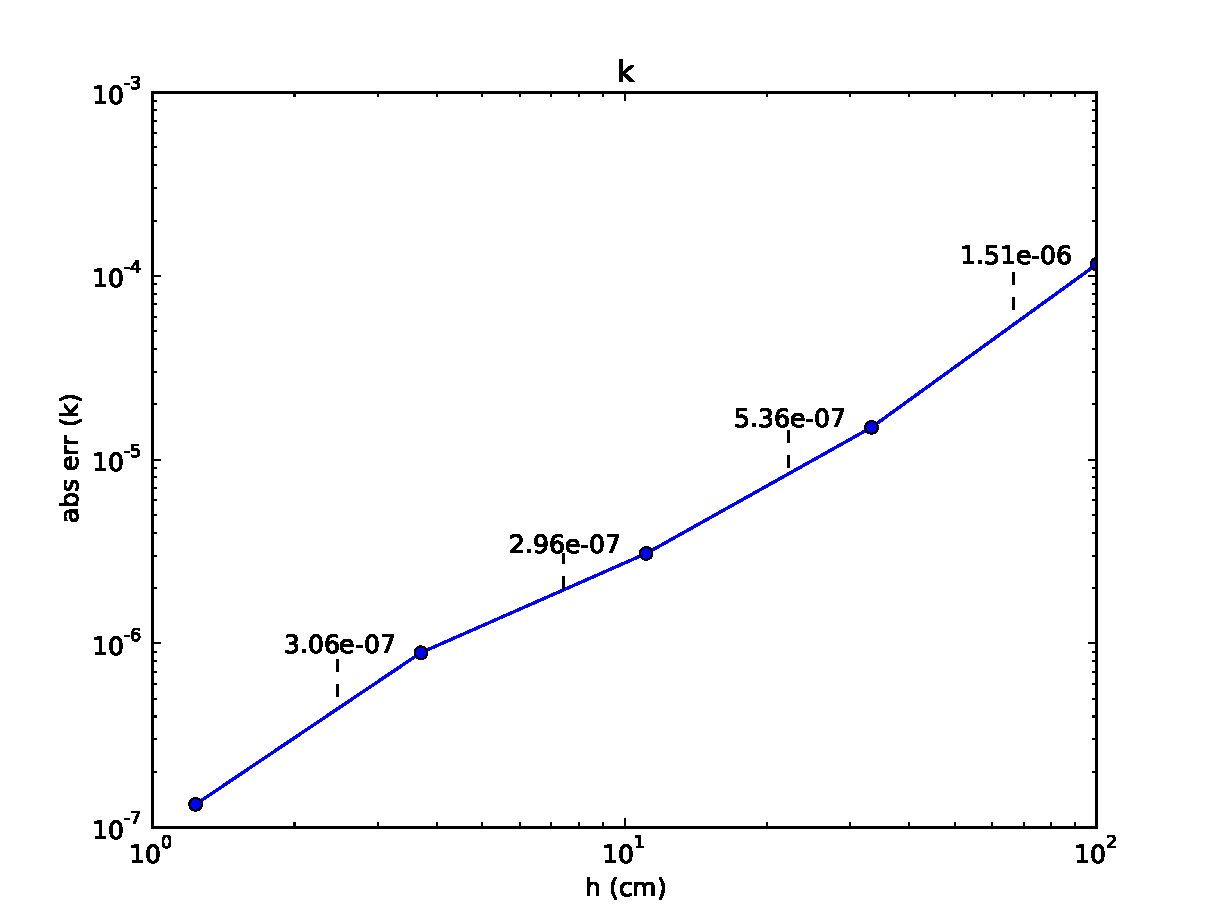
\includegraphics[width=0.7\textwidth]{k}
   \caption{Convergence of $k$-eigenvalue}
   \label{k}
\end{figure}
\begin{figure}[H]
\centering
   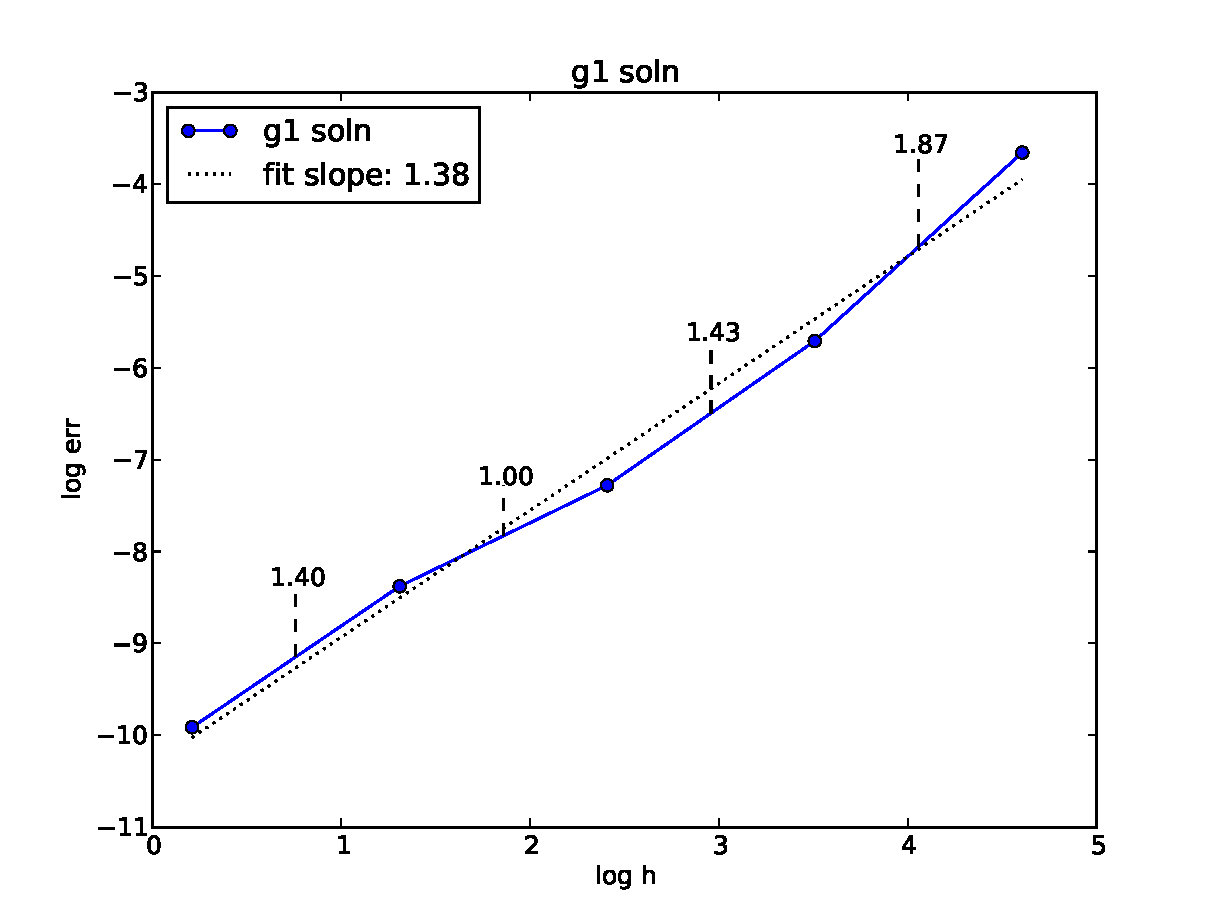
\includegraphics[width=0.7\textwidth]{g1}
   \caption{Convergence of Group 1 Flux}
   \label{g1}
\end{figure}
\begin{figure}[H]
\centering
   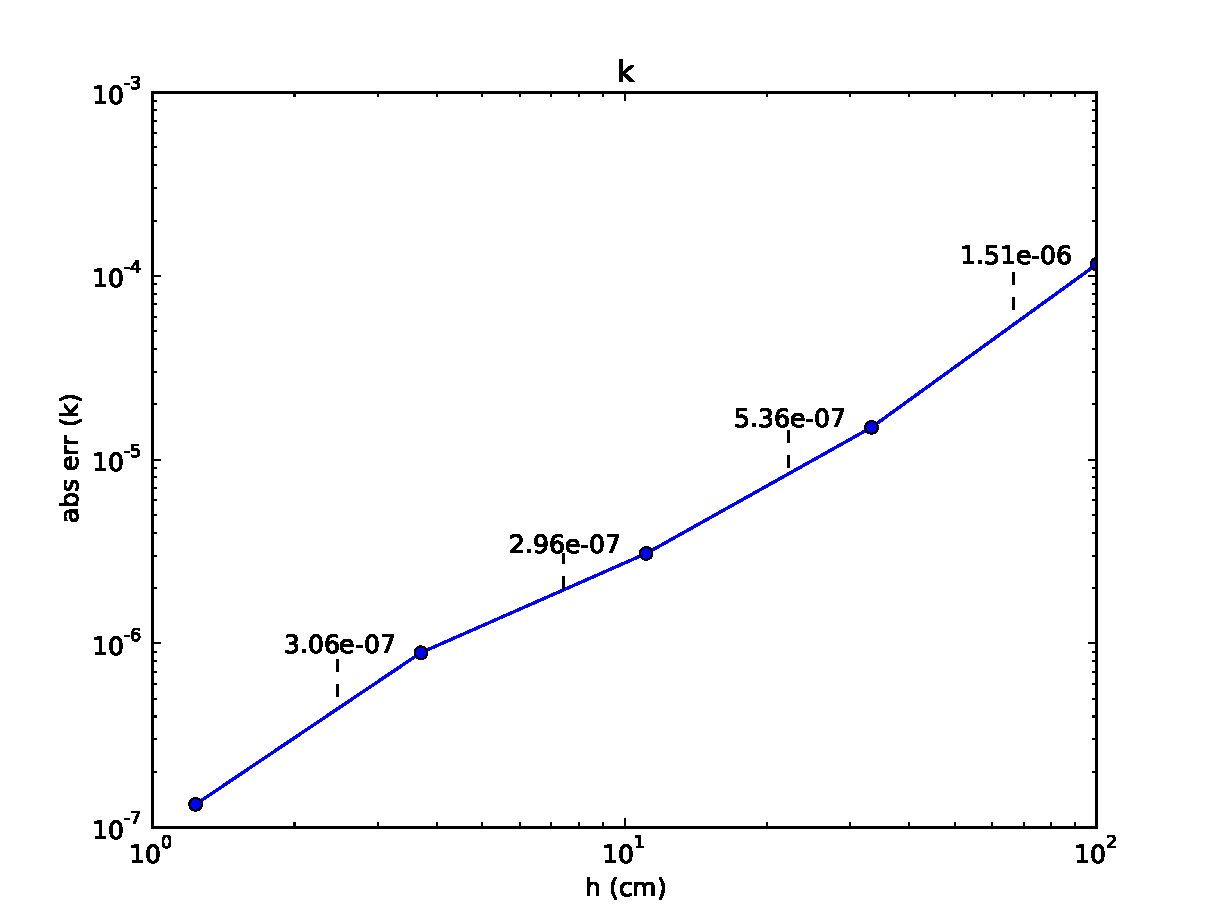
\includegraphics[width=0.7\textwidth]{k}
   \caption{Convergence of Group 2 Flux}
   \label{g2}
\end{figure}

\begin{table}[H]
\centering
\begin{tabular}{r r|l l l}
$h$ (cm) & $N_s$ & $\epsilon_{k}$ & $\epsilon_{g_1}$ & $\epsilon_{g_2}$ \\ \hline
1.23456790123 & 486 & 1.32959208754e-07 & 3.28397e-08 & 9.28242e-09 \\
3.7037037037 & 54 & 8.89666182058e-07 & 2.038143e-07 & 5.777665e-08 \\
11.1111111111 & 18 & 3.08556299755e-06 & 6.97189e-07 & 1.9768821e-07 \\
33.3333333333 & 6 & 1.49874897766e-05 & 3.3531505e-06 & 9.5092417e-07 \\
100.0 & 2 & 1.156465028e-04 & 2.607958593e-05 & 7.39625249e-06
\end{tabular}
\caption{Max absolute errors by grid refinement}
\label{tab}
\end{table}

\end{document}




\begin{figure}[h!]
\centering
  \begin{subfigure}[b]{0.45 \textwidth}
   \includegraphics[width=\textwidth]{FV_25}
   \caption{Finite Volume, $\Delta_x=25$ cm}
   \label{FV1}
  \end{subfigure}
  \begin{subfigure}[b]{0.45\textwidth}
   \includegraphics[width=\textwidth]{FV_004}
   \caption{Finite Volume, $\Delta_x=0.04$ cm}
   \label{FV3}
  \end{subfigure}
\end{figure}
